\documentclass[a4paper,11pt]{report}

% For the titlepage
\author{Aditya Dutta}
\title{Introduction to Complex Dynamics and the Mandelbrot Set}
\date{20th Aug, 2023}
\newcommand{\studentnumber}{18MS101}
\newcommand{\program}{BS-MS Dual Degree Program}
\newcommand{\supervisor}{Dr. Sushil Gorai}

% packages
\usepackage{mlmodern} % bolder fonts than normal
\usepackage{amsmath} % everything ams
\usepackage{amssymb}
\usepackage{amsthm}
\usepackage{mathtools}
\usepackage{hyperref} % for links (urls, cross-referencing, etc)
\hypersetup{
	colorlinks=true,
	linkcolor=blue,
	filecolor=blue,
	citecolor=black,
	urlcolor=cyan
}
\usepackage[nameinlink]{cleveref} % easy cross-referencing
\usepackage[margin=2.5cm]{geometry} % modify margins
\usepackage{graphicx} % include images
\usepackage{booktabs} % better latex tables
\usepackage{apacite} % for bibliography

% Gilles's castel's command for inkscape images
\usepackage{import}
\usepackage{xifthen}
\usepackage{pdfpages}
\usepackage{transparent}

\newcommand{\incfig}[1]{%
    \def\svgwidth{\columnwidth}
    \import{./figures/}{#1.pdf_tex}
}

% define basic theorem styles
\theoremstyle{plain}
\newtheorem{definition}{Definition}[section]
\newtheorem{theorem}{Theorem}[section]
\newtheorem{corollary}{Corollary}[theorem]
\newtheorem{lemma}[theorem]{Lemma}
\theoremstyle{remark}
\newtheorem*{remark}{Remark}

% custom commands
\newcommand{\fof[1]}{f^{\circ #1}}
\newcommand{\gog[1]}{g^{\circ #1}}
\newcommand{\fcof[1]}{f_c^{\circ #1}}
\newcommand{\ror[1]}{R^{\circ #1}}
\newcommand{\pop[1]}{P^{\circ #1}}
\newcommand{\bs}{\backslash}
\newcommand{\Cinf}{\hat{\mathbb{C}}}
\newcommand{\Finf}{F_\infty}

\linespread{1.3}

\begin{document}
\begin{titlepage}
	\makeatletter
	\begin{center}
		\textsc{Indian Institute of Science Education and Research, Kolkata} % institute
		\par \textsc{Department of Mathematics and Statistics} % department
		\par MS Project Report \program % program

		\vfill \hrule height .08em \bigskip
		\par\huge\@title\bigskip
		\par\Large\@author\,(\studentnumber)\bigskip
		\hrule height .08em\normalsize

		\vfill % add institute logo
		
\includegraphics[width=\textwidth,height=0.15\textheight,keepaspectratio]{logo}
		\vfill

		\begin{tabular}{ll}
			\toprule
			Supervisor: & \supervisor\\
			% Second assessor: & \secondassesor\\
			Date final version: & \today\\
			\bottomrule
		\end{tabular}

		\vfill
	\end{center}
	\makeatother
\end{titlepage}

\chapter{Introduction}
\section{The Spherical metric}
We begin by defining the extended complex plane, \( \Cinf \) simply as the union,\[
	\Cinf = \mathbb{C} \cup \{\infty\}
.\] 
To obtain, a metric on \( \Cinf \), we identify \( \mathbb{C} \) with the \( XY \) plane in \( \mathbb{R}^3 \).
And let \( S \) be the unit sphere centered at origin.\\
We then use the stereographic projection, \( \pi:z\mapsto z^* \)
by projecting each point \( z \) in \( \mathbb{C} \) linearly towards (or away) \( (0,0,1) \) until it
meets \( S \). We then define, \( \pi(\infty)=\infty \). In this way, \( \pi  \) is a bijective map
from \( \Cinf \) onto \( S \), and this is the reason why it \( \Cinf \) is also called the \emph{Complex or Riemann Sphere}.

We now define a natural metric on \( \Cinf \) using this stereographic projection as,\[
	\sigma(z,w)=|\pi(z)-\pi(w)|=|z^*-w^*|
.\] This is known as the \emph{Spherical metric} on \( \Cinf \) and we will use this metric mainly to define equicontinuity ahead.

\begin{center}
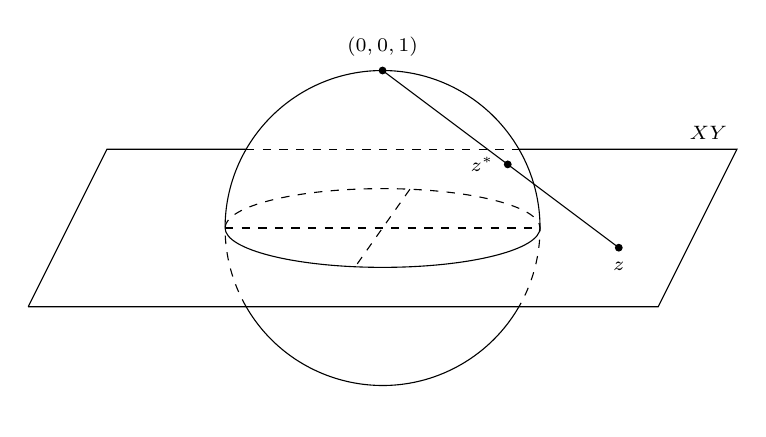
\begin{tikzpicture}
	\coordinate (A) at (3,-0.25);
	\coordinate (P) at (0,2);

	\draw (0:2cm)   arc[radius=2cm,start angle=0,end angle=180]
		  (210:2cm) arc[radius=2cm,start angle=210,end angle=330];
	\draw (180:2cm) arc[x radius=2cm, y radius=0.5cm, start angle=180,end angle=360];

	\draw [dashed] (210:2cm) 
		  arc[start angle=210,delta angle=-30,radius=2cm]
		  arc[start angle=180,delta angle=-180,x radius=2cm,y radius=0.5cm]
		  arc[start angle=0,delta angle=-30,radius=2cm];

	\draw [dashed] (80:2cm and 0.5cm) -- (260:2cm and 0.5cm);
	\draw [dashed] (150:2cm) coordinate(ul) -- (30:2cm) coordinate(ur);

	\draw (-4.5,-1) -- (3.5,-1) -- (4.5,1) node[anchor=south east] {\scriptsize$ XY $} -- (ur) (ul) -- (-3.5,1) -- (-4.5,-1);

	\draw (A) -- (P) coordinate[pos=0.47](B);
	\path (A) node[circle, fill, inner sep=1pt, label=below:{\scriptsize$ z $}]{};
	\path (B) node[circle, fill, inner sep=1pt, label=left:{\scriptsize$ z^* $}]{};
	\path (P) node[circle, fill, inner sep=1pt, label=above:{\scriptsize$ (0,0,1) $}]{};
	\draw [dashed] (-2,0) -- (2,0);
\end{tikzpicture}
	
\end{center}

\section{Rational maps}
\begin{definition}[\textbf{Rational maps}]
	A rational map is a function of the form, \[
		R(z)=\frac{P(z)}{Q(z)}
	,\] where \( P \) and \( Q \) are polynomials but not simultaneously zero polynomials.
	If \( Q(z)=0 \) and \( P \) is not the zero polynomial, then \( R \) is defined to be \( \infty \).
	Also, we define \( R(\infty) \) to be the limit of \( R(z) \) as \( z\to \infty \).
\end{definition}
We shall always assume \( P \) and \( Q \) are co-prime. We define the \textbf{degree} of a rational map \( R \) as, \[
	\deg(R)=\max\{\deg(P),\deg(Q)\}
.\] If \( R \) is a constant map (even \( \infty \)), we define, \( \deg(R)=0 \).

It is a crucial fact that if \( R \) is a rational function of degree \( d \), then \( R \) is a \( d \)-fold
map of \( \Cinf \) onto itself.


\section{Definition of Fatou and Julia sets in terms of equicontinuity}
\begin{definition}[\textbf{Fatou and Julia Sets}]
	Let \( R \) be a non-constant rational function. The Fatou set of \( R \) denoted by \( F(R) \) is 
	the maximal open subset of \( \Cinf \) on which \( \{\ror[n]\}\) is equicontinuous. The Julia set of \( R \),
	denoted by \( J(R) \) is the complement of \( F(R) \) in \( \Cinf \).
\end{definition}
By definition, \( F(R) \) is open and \( J(R) \) is compact.\\
They are denoted by simply \( F \) or \( J \) when the context is clear.

\section{Completely Invariant Components}
If \( f:X\to X \), then a subset \( D\subset X \) is:
\begin{itemize}
	\item \emph{forward invariant} under the map \( f \) if \( f(D)=D \).
	\item \emph{backward invariant} under the map \( f \) if \( f^{-1}(D)=D \).
	\item \emph{completely invariant} under the map \( f \) if it is both forward
		and backward invariant under \( f \) i.e. \( f(D)=D \) and \( f^{-1}(D)=D \).
\end{itemize}
Note that if \( f \) is surjective, i.e. \( f(X)=X \), then backward invariance implies complete invariance.
This is because, \( f(f^{-1}(D))=D \) if \( f \) is surjective. Hence, if \(f^{-1}(D)=D  \), we have \( f(D)=D \) i.e.
forward invariance.

\begin{theorem}
	If \( f:X\to X \) be a continuous, open and surjective map of a topological space \( X \) onto itself.
	If \( D\subset X \) is completely invariant under \( f \), then so are the complement \( X\bs D \), the interior \( D^0 \), 
	the boundary \( \partial D \) and the closure \( \overline{D}  \).
\end{theorem}
\begin{proof}
	Firstly, note that it is enough to prove backward invariance since \( f \) is surjective.\\
	It is trivial to see that \( X\bs D \) is completely invariant. 

	Now, since \( f \) is a continuous map,
	\( f^{-1}(D^0) \) is an open subset of \( f^{-1}(D)=D \). Hence, \( f^{-1}(D^0) \subset D^0 \). Now, since \( f \) is an open map,
	\( f(D^0) \) is an open subset of \( f(D)=D \). Hence, \( f(D^0) \subset D^0 \implies D^0 \subset f^{-1}(f(D^0)) \subset f^{-1}(D^0) \).
	Hence, \( f^{-1}(D^0)=D^0 \) and hence, \( D^0 \) is completely invariant.
	
	From the general fact for continuous maps, \( \overline{ f^{-1}(A)}\subset f^{-1}(\overline{A})  \). Hence, \( \overline{D}\subset f^{-1}(\overline{D})   \). Now, let \( x\in f^{-1}(\overline{D})  \) (or \( f(x)\in \overline{D}  \)). If \( x\not\in \overline{D}  \), then there exists and open set around \( x \), say \( U \) such that \( U\cap D=\phi \). Since \( f \) is an open map, \( f(U) \) is an open set containing \( f(x) \). Since, \( f(x)\in \overline{D}  \), \( f(U)\cap D\neq \phi \). But since, \( f^{-1}(D)=D \), \( f^{-1}(f(U)\cap D)\subset D \). But, \( f^{-1}(f(U)\cap D)\cap U\neq \phi \implies D\cap U\neq \phi\), which is a contradiction. Hence, \( \overline{D}=f^{-1}(\overline{D})   \). Hence, \( \overline{D}  \) is also completely invariant.

	Consequently, \( \partial D=\overline{D}\bs D^0  \) is also completely invariant.
\end{proof}

\begin{theorem}
	For any rational function \( R \), the Fatou and Julia sets of \( R \) i.e. \( F(R) \) and
	\( J(R) \) are completely invariant.
\end{theorem}
\begin{proof}
	First note that it is enough to prove only backward invariance because \( R \) is surjective.
	Also, we will only prove the complete invariance of \( F(R) \), the complete invariance of \( J(R) \) then follows
	from above theorem. We will use \( F \) to denote \( F(R) \).

	Let \( z_0\in R^{-1}(F) \) and let \( w_0=R(z_0)\in F \). By equicontinuity, for any \( \epsilon>0 \), \( \exists \delta>0 \) such
	that if \( \sigma(z,z_0)<\delta \), then for all \( n \in \mathbb{N} \), \( \sigma(\ror[n](w),\ror[n](w_0))<\epsilon \). By continuity of \( R \),
	there exists \( \delta'>w_0 \) such that if \( \sigma(z,w_0)<\delta' \), then \( \sigma(R(z),w_0)<\delta \) and hence,
	\( \sigma(\ror[n+1](z),\ror[n+1](z_0))<\epsilon \) for all \( n\in \mathbb{N} \). Hence, \( \{\ror[n+1]:n \in \mathbb{N}\} \) is equicontinuous 
	at \( z_0 \) and hence, so is \( \{\ror[n]:n \in \mathbb{N}\} \). Therefore, \( z_0 \in F \) and \( R^{-1}(F) \subset F \). 

	Now, let \( z_0 \in F \). To prove that \( z_0\in R^{-1}(F) \), we need to prove that \( R(z_0)\in F \). Let \( w_0=R(z_0) \).
	We have by equicontinuity, that for any \(\epsilon>0  \), \( \exists \delta>0 \) such that for all \( n \in  \mathbb{N} \), if \( \sigma(z,z_0)<\delta \), then \( \sigma(\ror[n+1](z),\ror[n+1](z_0))<\epsilon \). Now, \( N=\{z:\sigma(z,z_0)<\delta\} \) is an open set containing \( z_0 \)
	and hence, \( R(N) \) is an open set containing \( w_0 \). Now, if \( w\in R(N) \) then \( w=R(z) \) for some \( z\in N \). Hence, \[
		\sigma(\ror[n](w),\ror[n](w_0))=\sigma(\ror[n+1](z),\ror[n+1](z_0))<\epsilon
	.\] Hence, \( z_0\in R^{-1}(F) \) and \( F \subset R^{-1}(F) \).

Therefore, \( R^{-1}(F)=F \) and \( F(R) \) is completely invariant.
\end{proof} 

\begin{lemma}\label{thm1.3}
For any rational map \( R \) and a domain \( U \subset  \Cinf\), \( \partial R(U) \subset R(\partial U) \).
\end{lemma}
\begin{proof}
	Let \( w_0\in \partial R(U) \) such that it is approximated by \( R(z_n) \) for \( (z_n)_{n=1}^\infty \subset U \).
	Now, assume \( z_n\to z_0 \) (after taking a subsequence). Now, \( z_0 \) cannot lie in \( U \), otherwise \( R(z_0)=w_0 \in R(U) \).
	Since, \( R \) is an open map, \( R(U) \) is an open set and is disjoint from \( \partial R(U) \). Hence, \( z_0\in \partial U \)
	and \( R(z_0)=w_0 \in R(\partial U) \). Therefore, \( \partial R(U) \subset R(\partial U) \).
\end{proof}

\begin{lemma}\label{lem1.1}
	For a rational map \( R \), if \( F_1 \) and \( F_2 \) are two Fatou components and \( R \)
	maps a point of \( F_1 \) to a point of \( F_2 \), then \( R(F_1)=F_2 \).
\end{lemma}
\begin{proof}
Clearly, \( R(F_1)\subset F_2 \) because of forward invariance of \( F \) under \( R \) and since \( F_1 \) and \( F_2 \)
are connected components of \( F \). If \( R(F_1)\neq F_2 \), then \( \exists z \in \partial F_1 \) such that \( R(z)\in F_2 \) and
this is not possible as \( z\in \partial F_1\implies z\in J \) and \( J \) is completely invariant. Hence, \( R(F_1)=F_2 \).
\end{proof}

\begin{theorem}\label{thm1.4}
	The unbounded Fatou component of a polynomial \( P \), i.e. the Fatou component containing \( \infty \)
	is a completely invariant Fatou component. It is denoted by \( F_\infty(P) \) or simply \( F_\infty \) when
	the context is clear.
\end{theorem}
\begin{proof}
	First note that since \( P(\infty)=\infty \), we have \( P(F_\infty)=F_\infty \) by the above lemma. Hence, \( F_\infty \subset P^{-1}(F_\infty) \).
	Now assume, some point \( z_0\in P^{-1}(F_\infty) \) but \( z_0\not\in F_\infty \). By backward invariance of \( F \),  \( z_0\in F' \),
	where \( F' \) is some other Fatou component. Again, \( P(F')=F_\infty \) by above lemma. But for polynomials, we have \( P^{-1}(\infty)=\{\infty\}\). Hence, \( \infty \in F' \) and \( F' \) must be \( F_\infty \) itself. Therefore, \( P^{-1}(F_\infty)=F_\infty \) and \( F_\infty \) is completely invariant under \( P \).
\end{proof}

\begin{theorem}
	Let \( R \) be rational map and let \( E \) be a finite set which is completely invariant under \( R \). 
	Then \( E \) has atmost two elements.
\end{theorem}
\begin{proof}
	Suppose \( E \) has \( k \) elements. Now, \( R \) acts as a permutation of \( E \) and hence for some integer \( s \),
	\( \ror[s] \) acts as an identity map on \( E \). Now, suppose \( \ror[s] \) has degree \( d \). It follows that for any \( z_0\in E \),
	\( \ror[s](z)=z_0 \) has solution \( z_0 \) with multiplicity \( d \). Applying the Riemann-Hurwitz formula, (in the next section) \[
		k(d-1)\le 2d-2
	\] and hence, \( k\le 2 \).
\end{proof}


\section{Valency and the Riemann-Hurwitz formula}
Let \( f \) be a holomorphic map on the complex plane. Then, near a point \( z_0 \), \( f \) has the Taylor expansion,\[
	f(z)=f(z_0)+a_k(z-z_0)^k+\ldots 
,\]  where \( a_k\neq 0 \) and \( k\ge 1 \). Then, we define the valency of \( f \) at \( z_0 \),
\( v_f(z_0)=k \).

For \( f:X\to Y \) where \( X \) and \( Y \) are Riemann surfaces, we have local analytic co-ordinates near \( z_0 \)
and \( f(z_0) \) such that \( f \) has the form \( f(z)=a_kz^k+\ldots  \), (\( a_k\neq 0 \) and \( k\ge 1 \))
then again we define the valency of \( f \)
at \( z_0 \) as \( v_f(z_0)=k \). The valency is independent of the choice of co-ordinates.

\begin{definition}[Deficiency]
	We define the deficiency of \( f \) over a set \( A \) as, \[
		\delta_f(A)=\sum_{z\in A} (v_f(z)-1)
	.\] 
\end{definition}

\begin{theorem}[\textbf{Generalized Riemann-Hurwitz formula}]
	Let \( X \) and \( Y \) be Riemann surfaces and \( f:X\to Y \) be a complex analytic map of degree \( d \). Then,
	\[
		\chi(X)+\delta_f(X)=d\chi(Y)
	,\] where \( \chi(X) \) denotes the Euler characteristic of \( X \).\\
	For a compact, connected and orientable surface \( S \), the Euler characteristic \( \chi(S)=2-2g \),
	where \( g \) is the genus of \( S \). Hence, if \( X \) and \( Y \) are compact Riemann surfaces,
	we get the following formula (after multiplying both sides by \( -1 \)),\[
		2g(X)-2=d(2g(Y)-2)+\delta_f(X)
	.\] 
\end{theorem}

\begin{theorem}[\textbf{Riemann-Hurwitz Formula} (version 1)]
Now, genus of a sphere is zero and hence, \( g(\Cinf)=0 \).
For a rational map, which is a \( d \)-fold map of the complex sphere onto itself, we have,
\begin{align*}
	\implies & 2g(\Cinf)-2=d(2g(\Cinf)-2)+\delta_R(\Cinf)\\
	\implies &\delta_R(\Cinf)=2d-2\\
	\implies &\sum_{z\in \Cinf}(v_R(z)-1)=2d-2
.\end{align*}
\end{theorem}

\begin{theorem}[\textbf{Riemann-Hurwitz Formula}  (version 2)]
	Let \( F_0 \) and \( F_1 \) be components of the Fatou set \( F \) of a rational map \( R \)
	and \( R \) maps \( F_0 \) into \( F_1 \). Then, for some integer \( m \), \( R \) is an \( m \)-fold
	map of \( F_0 \) onto \( F_1 \) and \[
		\chi(F_0)+\delta_R(F_0)=m\chi(F_1)
	.\] 
\end{theorem}

\section{Equicontinuity and Normality}
There is another criterion that we use more in practice to define Fatou sets.
\begin{definition}[\textbf{Normal Families}]
	A family of maps, \( \mathcal{F} \) of maps from metric space \( (X_1,d_1) \) to \( (X_2,d_2) \) is said to be a normal family in \( X_1 \),
	if every infinite sequence of function in \( \mathcal{F} \) has a subsequence which converges locally uniformly on \( X_1 \).
\end{definition}

The Arzela-Ascoli theorem connects equicontinuity and normality. This is one of the many forms of the theorem, which is suitable for our use.
\begin{AAT}
	Let \( D \) be a domain on the complex sphere and let \( \mathcal{F} \) be a family of continuous maps defined on \( D \).
	Then, \( \mathcal{F} \) is equicontinuous in \( D \) if and only if  it is a normal family in \( D \).
\end{AAT}
Thus, we can redefine the Fatou set of \( R \) as the maximal open set of \( \Cinf \) 
on which the family \( \{\ror[n]\} \) is normal.

\begin{theorem}[\textbf{Vitali's Theorem}]
		Let \( D \) be a subdomain of complex sphere. Suppose \( \{f_n\}_{n\in\mathbb{N}} \)	be a family of analytic maps normal in \( D \). Also suppose, \( \{f_n\} \) converges pointwise on some subset \( W\subset D \) such that \( W \) contains a limit point in \( D \). Then, \( f(z):=\lim_{n \to \infty} f_n(z), z\in W \) extends to an analytic function \( F \) on \( D \) and \( f_n\to F \) locally uniformly in \( D \).
\end{theorem}
\begin{proof}
	As \( \{f_n\} \) is a normal family, there is a subsequence of \( (f_n) \) which converges locally uniformly in \( D \)
	to some analytic function \( F \) and \( F=f \) on \( W \).

	Now, assume \( (f_n) \) fails to converge locally uniformly to \( F \) on \( D \). Then, there is some subsequence \( (g_n) \)
	of \( (f_n) \) and \( \epsilon>0 \) such that for all \( n \) and all \( z\in K \),\[
		\sigma(g_n(z),F(z))\ge \epsilon
	.\] But again by normality, there is a subsequence \( (h_n) \) of \( (g_n) \) which converges locally uniformly in \( D \)
	to some analytic function \( h \). Clearly, \( h=F=f \) on \( W \) and since \( W \) has a limit point in \( D \),
	\( h=F \) throughout \( D \) by the Identity theorem. It follows that, \[
		\sigma(h_n(z),F(z))\to 0
	\]  uniformly in \( K \). This is a contradiction as \( (h_n) \) is a subsequence of \( (g_n) \).
	Hence, \( (f_n) \) converges locally uniformly to \( F=f \) on \( D \).
\end{proof}

\begin{corollary}\label{lem1.2}
	If \( \alpha \) is a (super)-attracting fixed point of a rational map \( R \) and \( F_\alpha \) is the
	Fatou component containing \( \alpha \) then \( \ror[n](z)\to \alpha \)
	locally uniformly in \( F_\alpha \).
\end{corollary}

We now state one of the most important theorem for normal families, the \emph{Montel's Fundamental Normality Criterion}.
It provides us with a very easy way to check if some family of maps is normal on a domain of the complex sphere.
\begin{theorem}[\textbf{Montel's Fundamental Normality Criterion}]
	Let \( \mathcal{F} \) be a family of maps, each analytic in a domain \( D \) of the complex sphere.
	Suppose \( \exists m>0 \) and for each \( f\in \mathcal{F} \), three distinct points \( a_f,b_f \) and \( c_f \) such that,
	\begin{enumerate}
		\item \( f(D) \) does not contain \( a_f,b_f \) and \( c_f \),
		\item \(\min\{\sigma(a_f,b_f),\sigma(b_f,c_f),\sigma(c_f,a_f)\}\geq m\),
	\end{enumerate}
	then \( \mathcal{F} \) is normal in \( D \).
\end{theorem}

\section{Exceptional points and minimality of the Julia set}
\begin{theorem}[\textbf{Minimality of \( J \)}]
	Let \( R \) be a rational map with \( \deg(R)\ge 2 \) and suppose that \( E \) is a closed, completely invariant
	subset of the complex sphere. Then either,
	\begin{enumerate}
		\item \( E \) has atmost two elements and \( E \subset E(R) \subset F(R) \).
		\item \( E \) is infinite and \( J(R) \subset E \).
	\end{enumerate}
\end{theorem}
\begin{proof}
	We know that either \( E \) has atmost two points or it is infinte. If \( E \) is finite, then \( E \) contains
	only exceptional points which lie in \( F(R) \). Now, suppose \( E \) is infinite. As \( E \) is completely invariant, so
	is its complement, say \( G \). Hence, \( \ror[n] \) maps \( G \) into itself for each \( n \in \mathbb{N} \). Hence, applying 
	Montel's Fundamental Normality Criterion, while choosing \( a_f,b_f \) and \( c_f \) to be any three points in \( E \),
we see that \( \{\ror[n]\} \) is a normal family in \( G \). Hence, \( G \subset F \implies J \subset G^c=E \).
\end{proof}
\noindent This result can also be stated as:\\
\textbf{\( J \) is the smallest, closed completely invariant set with atleast three points.}

\begin{corollary}\label{thm1.2}
	If \( R \) is a rational function, with \( \deg(R)\ge 2 \), and \( F_0 \) is
	a completely invariant Fatou component of \( R \), then, \( \partial F_0=J \).
\end{corollary}
\begin{proof}
	As \( F_0 \) is completely invariant, so is \( \overline{F_0}  \). By minimality of \( J \), \( J\subset \overline{F_0}  \).
	As \( J \) is disjoint from \( F_0 \), \( J=\partial F_0 \).
\end{proof}

\section{Connectivity}
\begin{definition}[Connectivity]
	The connectivity of a domain \( D \subset \Cinf \) is defined as the number
	of components of \( \partial D \).
\end{definition}

\begin{theorem}\label{thm1.1}
	The following are equivalent for a domain \( D\subset \Cinf \):
	\begin{enumerate}
		\item \( D \) is simply connected.
		\item \( D^c \) is connected.
		\item \( \partial D \) is connected or \( c(D)=1 \).
	\end{enumerate}
\end{theorem}
\begin{proof}
	\( D^c \) being connected can be taken as the definition of \( D \) being simply connected, as it is done by Ahlfors \parencite{ahlfors}.
	Later it is this definition of simply connected, which is used to prove the Riemann mapping theorem, which proves biholomorphism
	between simply connected sets and the unit disc which is actually simply connected.

	We will prove the equivalence of \emph{1} and \emph{3}.

	If \( D \) is not simply connected, then there is a simple closed curve \( \gamma \) in \( D \) which 
	separtes the complement of \( D \), proving that \( \partial D \) is disconnected.

	Now, suppose that \( \partial D \) is disconnected. Then there is a simple closed curve \( \gamma \) which
	separtes \( \partial D \) into two disjoint subsets \( A \) and \( B \). Since, \( D \) is path-connected and
	\( D \) is arbitrarily close to \( A \) and \( B \), \( D \) intersects \( \gamma \). By construction, \(\gamma\) does
	not intersect \( \partial D \) and hence, \( \gamma\) lies in \( D \). Thus, \( A \) and \( B \) lie in different
	components of the complement of \( D \) and hence, \( D \) cannot be simply connected.
\end{proof}

\noindent \textbf{Note:} If \( D \) is simply connected, we have \( c(D)=1 \) and \( \chi(D)=1 \).\\
More generally, \( \chi(D)=2-c(D) \).



\chapter{Behaviour of analytic functions near fixed points}
\section{Behaviour near parabolic fixed points}
A point \( p \) is called a parabolic fixed point of \( f \)
if \( f(p)=p \) and \( f'(p)=e^{2\pi i t} \), where \( t \)
is a rational number.

% TODO: Add previous theorem
% TODO: Add definition of petals
% TODO: Add figure for petals

\begin{theorem}[\textbf{The Petal Theorem}]
Suppose that an analytic map \( f \) has the form:\[
	f(z)=z-z^{p+1}+\mathcal{O}(z^{2p+1})
\] near the origin. Then for sufficiently small \( t \),
\begin{enumerate}
	\item \( f \) maps each \( \Pi_k(t) \) into itself;
	\item \( \fof[n](z)\to 0 \) uniformly on each petal;
	\item \( \arg(\fof[n](z))\to 2k\pi /p \) locally uniformly on each petal;
	\item \( f:\Pi_k(t)\to \Pi_k(t) \) is conjugate to a translation.
	\item \( |f(z)|<|z| \) on a neighbourhood of the axis of each petal;
\end{enumerate}
\end{theorem}

\begin{proof}
	For \( 0<r_0<1 \), define the sector \( S_0 \), \[
		S_0=\{re^{i\theta}:0<r<r_0,|\theta |<\pi /p \}
	\] and the region \( W \), \[
	W=\{re^{i\theta }:r>\frac{1}{r_0^p},|\theta |>\pi\}
	.\] 
	It is clear that the map \( \sigma:z\mapsto \frac{1}{z^p} \) is a biholomorphism
	of \( S_0 \) onto \( W \) with \( \sigma^{-1}:W\to S_0 \) given by \( \sigma^{-1}(w)=1 /w^{\frac{1}{p}} \).
	The branch of \( p \)-th root that we select determines which sector of width \( 2\pi /p \), the inverse map
	maps to. (The other sectors being \( S_k=\{0<r<r_0,|\theta -2k\pi /p|<\pi /p \} \).)

	Now, the conjugate map of \( f \) on \( W \) is given by,\[
		g(w)=\sigma f \sigma ^{-1}(w)=f(w^{-\frac{1}{p}})^{-p}
	.\]

	This just replaces the action of \( f \) on \( S \) by \( g \) on \( W \),
	and we have the following commutative diagram:

	%TODO: add commutative diagram and solve for the estimates of g

	\noindent Hence, we have the following estimates 
	for \( g \) which will be crucial in everything that will follows:
	\begin{align}
		g(w)&=w+p+A /w+\theta (w),\text{ where \( A \) is a constant and} \label{eqn3.1}\\
		|\theta (w)|&\le B /|w|^{1+\frac{1}{p}}, B>0 \label{eqn3.2}
	.\end{align}

	\noindent Choose any \( K \) satisfying \[
	K>\max\{ 1 /r_0^p,3(|A|+B) \}>1 \text{ (as \( r_0<1 \))}
	\]  and let, \[
		\Pi=\{x+iy:y^2>4K(K-x)\}
	.\] Clearly, \( \Pi \) is bounded by a parabola and \( \Pi\subset W \).

	We have chosen this subset \( \Pi\subset W \) because we will show that \( \Pi \)
	is nothing but the conformal image of \( \Pi_0(t) \) under \( \sigma \) (for a suitable \( t \)) and
	\( g \) satisfies all the corresponding conditions that \( f \) should satisfy on \( \Pi_0(t) \) according to the
	theorem.\\
	\vspace{1pt}

	\noindent \textbf{Claim.} \( \Pi \) is the conformal image of \( \Pi_0(t) \) under \( \sigma \) for a suitable \( t \).\\
	The easiest way to see this is using polar coordinates. We write, \( z=re^{i\theta } \) for \( z\in S \) 
	and \( w=\rho e^{i \phi } \) for \( w\in W \). Then, \( \rho=\frac{1}{r^p} \) and \( \phi=-p\theta  \).
	
	Now, we need to express \( \Pi  \) in polar co-ordinates. To do so, we notice that points on the parabola are given by \[
		\rho \text{ (distance from focus i.e. \( 0 \))}= 2K-\rho \cos \phi \text{ (distance from directrix i.e. \( y=2K \))}
	.\] 
	Therefore, points on \( \Pi \) are given by \[
		\rho > 2K-\rho \cos \phi 
	.\] 
	% TODO: Add figure
	Hence, \[
		\Pi=\{\rho e^{i\phi }:2K<\rho (1+\cos \phi )\}
	.\] Now, let \( \Omega=\sigma^{-1}(\Pi) \).
	Then, \( \Omega \) is given by \[
		\Omega=\{re^{i \theta }:2Kr^p<1+\cos (p\theta )\}
.\] Hence, \( \Omega=\Pi_0\left(\frac{1}{2K}\right) \).

\begin{lemma}
	\( g \) satisfies the following properties on \( \Pi \):
	\begin{enumerate}
		\item \(\Pi\) is forward invariant under \( g \).
		\item \( \gog[n](w)\to \infty \) uniformly on \( \Pi \).
		\item \( \arg(\gog[n](w))\to 0 \) locally uniformly on \( \Pi \).
		\item \( g:\Pi\to \Pi \) is conjugate to a translation.
	\end{enumerate}
\end{lemma}
\begin{proof}\text{}\\
	\noindent \textbf{\emph{1.}} We write, \[
		w=x+iy,\,\, g(w)=X+iY,\,\, A /w+\theta(w)=a+ib
	.\] 
	From \Cref{eqn3.1}, we obtain,
	\begin{align*}
		X+iY=(x+iy)+p+(a+ib)\\
	\implies X=x+p+a\text{ and }Y=y+b
	.\end{align*}
	Now, if \( w\in \Pi  \),
	\begin{align*}
		Y^2-4K(K-X)&=(y+b)^2-4K(K-x-p-a)\\
				   &=[y^2-4K(K-x)]+b^2+2yb+4K(a+p)\\
				   &> 4Kp+(2yb+4Ka)\\
				   &\ge |4Kp- |2yb+4Ka| |
	.\end{align*}
	Now, for \( w\in\Pi \), \( |w|>K>1 \). Hence we get,
	\begin{align}
		|w||A /w+\theta (w)|\le |w| (|A| /|w|+ B /|w|^{1+\frac{1}{p}})=|A|+B /|w|^{\frac{1}{p}}<|A|+B \label{eqn3.3}
	\end{align}
	(since for \( |w|>1 \), \( |w|^{\frac{1}{p}}>1 \)).  Therefore,
	\begin{align*}
		|2yb+4Ka|&\le 2|yb|	+4K|a|\\
				 &\le 2|y| |b|+4 K |a| \\
				 &\le 2|w| |a+ib| +4 |w| |a+ib| \\
				 &=6|w| |a+ib|\\
				 &<2K<2Kp
	.\end{align*}
	Therefore, we see that \( Y^2-4K(K-X)>0 \) and hence, \( g(w)\in \Pi \) for \( w\in \Pi \).
	Hence, \( \Pi \) is forward invariant under \( g \).\\
	\vspace{1pt}

	\noindent \textbf{\emph{2.}} Now, we will prove a stronger statement that for any \( t>0 \)
	\( g \) maps \( \Pi+t \) into \( \Pi+t+p /2 \). This is simply because, for \( w\in\Pi+t \),
	we have, \( y^2-4K(K+t-x)>0 \). Hence,
	\begin{align*}
		Y^2-4K(K+t+p /2-X)&=[y^2-4K(K+t-x)]+b^2+2yb+4K(a-p /2)\\
		&> 2Kp+(2yb+4Ka)\\
		&\ge |2Kp - |2yb+4Ka| |\\
		&>0
	.\end{align*}
	Therefore, if \( w\in\Pi \), \( \gog[n](w)\in \Pi+np /2 \). Hence, \( |\gog[n](w)|>\sqrt{n}  \).
	This is simply because, \( K+np /2>1+n /2>\sqrt{n}  \) and hence \( \Pi+np /2 \) is disjoint from the
disc \( \{|z|\le \sqrt{n} \} \).

Hence, \( \gog[n](w)\to \infty \) uniformly on \( \Pi \).\\
\vspace{1pt}

\noindent \textbf{\emph{3.}} Firstly, we see that, \[
	\gog[k](w)=g(\gog[k](w))=\gog[k](w)+p+A /\gog[k](w)+\theta (\gog[k](w))
.\] 
By expanding the first term again and again, we obtain,
\begin{align}
	\gog[n](w)&=w+np+ \sum_{k=0}^{n-1} \left(\frac{A}{\gog[k](w)}  +\theta(\gog[k](w))\right) \label{eqn3.4}
.\end{align}

Also note that form \Cref{eqn3.3}, we have, \[
	|A /w+\theta (w)|<(|A|+B) /K <\frac{1}{3}
.\] 

Let \( Q \) be a compact subset of \( \Pi \). From now, we will assume that \( w\in Q \) and we will use
\( C_1,C_2,C_3,\ldots  \) to denote positive constants which will be dependent on \( Q \).

Hence,
\begin{align*}
|g(w)|=|w+p+A /w+\theta (w)|&\ge ||w+p|-|A /w+\theta (w)| |\\
								&= |w+p|-|A /w+\theta (w)|\\
								&\ge |w|+p-\frac{1}{3}
.\end{align*}
Therefore, we obtain, \[
	|\gog[n](w)|\ge |w|+n(p-1 /3)\ge C_1+C_2n
.\] 
(Here, \( C_1=\min\{|w|:w\in Q\}>0 \) and \( C_2=p-\frac{1}{3}>0 \).)\\
We can select \( C_3 \) large enough such that
\begin{align}
	|\gog[n](w)|\ge C_3 n\label{eqn3.5}.
\end{align}
Next, with \Cref{eqn3.2}, and the above inequality, we get,
\begin{align}
	|\theta (\gog[n](w)|\le B /|\gog[n](w)|^{1+\frac{1}{p}}\le C_4 /n^{1+\frac{1}{p}}\label{eqn3.6}
.\end{align}

Finally, combining the above two inequalities and \Cref{eqn3.4}, we obtain,
\begin{align*}
	|\gog[n](w)-np|&\le |w|+|A /w+\theta (w)|+\frac{|A|}{C_3}\sum_{k=1}^{n-1} \frac{1}{k}+C_4\sum_{k=1}^{n-1} \frac{1}{n^{1+\frac{1}{p}}}\\
				   &< C_5+C_6\sum_{k=1}^{n} \frac{1}{k}
.\end{align*}
(Here, \( C_5=\max\{|w|:w\in Q\}+\frac{1}{3}+C_4\sum_{n=1}^{\infty}  1 /n^{1+\frac{1}{p}} \) and \( C_6=|A| /C_3\).)\\
We can select \( C_7 \) large enough such that
\begin{align}
	|\gog[n](w)-np|<C_7 \log n \label{eqn3.7}
.\end{align}

\begin{remark}
	The above inequality follows from the fact that, if \( H_n=\sum_{k=1}^n \frac{1}{k} \), then \( H_n-\log n\to \gamma \).
	(\( \gamma \) is known as the Euler's constant).
	So, we have that
	\begin{align*}
		P+QH_n &=P+Q(\log n+\gamma +\epsilon_n), \text{where \( \epsilon_n\to 0 \)}\\
			   &\le Q\log n+(P+Q\max\{\epsilon_n\}+Q\gamma)\\
			   &=Q\log n+R\\
			   &<S \log n
	\end{align*} for \( S \) large enough.
\end{remark}

\begin{figure}[ht]
    \centering
    \incfig{argogn}
    \caption{}
    \label{argogn}
\end{figure}
From, \( |\gog[n](w)-np|<C_7\log n \), it follows that \( |\arg(\gog[n](w)|<\sin ^{-1}\left(\frac{C_7\log n}{np}\right) \)
for \( n \) large enough. Hence, \( \arg(\gog[n](w))\to 0 \) uniformly on \( Q \), and consequently, locally uniformly on \( \Pi \).\\
\vspace{1pt}

\noindent\textbf{\emph{4.}} Define, \[
	u_n(w)=\gog[n](w)-np-(A /p)\log n
.\] 
\noindent\textbf{Claim.} \( u_n(w) \) converges locally uniformly on \( \Pi \) to a holomorphic function \( u \), that is one-to-one
on \( \Pi \).
\begin{align*}
	u_{n+1}(w)-u_n(w)&=[\gog[n+1](w)-\gog[n](w)]-p-(A /p)\log \left(\frac{n+1}{n}\right)
.\end{align*}
From \Cref{eqn3.2}, we obtain, 
\begin{align*}
	u_{n+1}(w)-u_n(w) &= \!\begin{multlined}[t]
							[\gog[n](w)+p+A /\gog[n](w)+\theta(\gog[n](w))-\gog[n](w)]\\
							 -p-(A /p)\log (1+1 /n)
						 \end{multlined}\\
					  &= A /\gog[n](w)+\theta (\gog[n](w))- (A /p)\log (1+1 /n)\\
					  &= A(1 /\gog[n](w)-1 /np)+\theta (\gog[n](w))+(A /p)(1 /n-\log (1+1 /n))
.\end{align*}
Now, let \( Q \) is a compact subset of \( \Pi \) and \( w\in Q \).
We need to prove that \( u_n \) converges uniformly in \( Q \). From the above equation, to prove
that \( u_n \) converges uniformly in \( Q \), we need to show that each of the following series converges uniformly in \( Q \):\[
	\sum_n |1 /\gog[n](w)-1 /np|,\,\,\sum_n|\theta (\gog[n](w)),\,\,\sum_n|1 /n-\log (1+1 /n)|
.\] 
Let us look at the first series. We have, (using \Cref{eqn3.5,eqn3.7}) \[
	|1 /\gog[n](w)-1 /np|=\frac{|\gog[n](w)-np|}{|\gog[n](w)|np}\le \frac{C_7 \log n}{C_3 n^2 p}=C_8\log n /n^2
.\] 
(Here \( C_8=C_7 /(pC_3) \)).

\noindent From \Cref{eqn3.6}, it is clear that \( \sum_n |\theta(\gog[n](w))| \) converges.

\noindent Now, \( 0<x-\log (1+x)\le   x^2 \) for \( x>0 \). \\
This is because, it is zero at \( x=0 \)
and \( \frac{d}{dx}(x-\log (1+x))=1-\frac{1}{1+x}>0 \) for \( x>0 \).\\
Also, \( x^2-x+\log (1+x) \) is zero at \( x=0 \) 
and \( \frac{d}{dx}(x^2-x+\log (1+x))=2x-1+\frac{1}{1+x}>0 \) for \( x>0 \).

Putting \( x=\frac{1}{n} \), we get, \[
	|1 /n-\log (1+ 1 /n)|<1 /n^2
.\] 
Therefore, \( u_n\) converges locally uniformly to some holomorphic function \( u \) on \( \Pi \).\\
Now, from \( u_n(w)=\gog[n](w)-np-(A /p)\log n \), we get that, 
\begin{align*}
	(n+1)p+(A /p)\log (n+1)+u_{n+1}(w)&=\gog[n+1](w)\\
									  &=\gog[n](g(w))\\
									  &=np+(A /p)\log n+u_n(g(w))\\
	\implies p+(A /p)\log (1+1 /n)+u_{n+1}(w)&=u_n(g(w))
.\end{align*}
Taking limit \( n\to \infty \), we get, \[
	p+u(w)=u(g(w))
.\] 
Since \( f \) is injective near the origin, \( g \) is injective on \( \Pi \),
(if \( K \) is chosen large enough). Therefore, \( \gog[n] \) is injective on \( \Pi \)
and hence, so is \( u_n \). By Hurwitz Theorem, \( u \) is either injective or constant, but it
is clearly not a constant since it satisfies the above equation.

This shows that \( g:\Pi\to \Pi \) is conjugate to the map \( z\mapsto z+p \) of \( u(\Pi) \) into
itself.
\end{proof}

Coming back to our original theorem, we see that since \( g \) maps \( \Pi \) into itself, \( f\)
also maps each \( \Pi_k(t) \) into itself.

Now since, \( |\gog[n](w)|>\sqrt{n}  \) for all \( w\in\Pi \), 
\( |\sigma \fof[n]\sigma^{-1}(w)|\to \infty \)
uniformly on \( \Pi \).

\section{Behaviour near attracting fixed points}

\section{Behaviour near super-attracting fixed points}
We will study the behaviour of analytic maps near super-attracting fixed
points in the next chapter under Bottcher's theorem.

\end{proof}

\chapter{Bottcher's Theorem and its extension}
\section{Bottcher's Coordinates}
A fixed point $p$ is called a super-attracting fixed point of $f$ if $f^{\prime}\left(p\right)=0$.\\
If $p$ is a super-attracting fixed point for $f$, we can conjugate the map such that $z=0$ becomes our super-attracting fixed point.

Thus, our map takes the form $$f(z)=a_{n} z^{n}+a_{n+1} z^{n+1}+\ldots$$ in a neighbourhood of 0 , with $n \geq 2$ and $a_{n} \neq 0$. Here the integer $n$ is the \emph{local degree} or \emph{valency} of \( f \) at \( 0 \).

\begin{theorem}[\textbf{Bottcher's Theorem}]
	With $f$ as above, $\exists$ a local holomorphic change of coordinates $w=\phi(z)$, with $\phi(0)=0$, which conjugates $f$ to $w \mapsto w^{n}$ throughout some neighbourhood of 0 .\\
Furthermore, $\phi$ is unique upto multiplication by an $(n-1)$ th root of unity.
\end{theorem}

\begin{proof}
	\textbf{Existence.} Let $c \in \mathbb{C}$ be such that $c^{n-1}=a_{n}$. Then, the linearly conjugate map $c f(z / c)$ will have leading coefficient +1 . Thus, without loss of generality, we will assume that our map $f$ has the form, $$f(z)=z^{n}(1+b_{1} z+b_{2} z^{2}+\ldots)=z^{n}(1+\eta(z)), \text{ where }\eta(z)=\left(1+b_{1} z+b_{2} z^{2}+\ldots\right).$$
Choose $r \in\left(0, \frac{1}{2}\right)$ such that $|\eta(z)|<\frac{1}{2}\,\, \forall z \in \mathbb{D}_{r}$. This can be done since $\eta(0)=0$ and $\eta$ is continuous.

\noindent On this disc, we have two properties of $f$ :
\begin{enumerate}
  \item $f$ maps this disc into itself:
	We have, $|f(z)|=\left|z^{n}\right||1+\eta(z)| \leq|z|^{n}(1+|\eta(z)|)<\frac{3}{2}|z|^{n} \leq \frac{3}{2^{n}}|z| \leq \frac{3}{4}|z|$ $\forall z \in \mathbb{D}_{r}$. Here we are using the fact that $n \geq 2,|z|<\frac{1}{2}$ and $|\eta(z)|<\frac{1}{2}$ on $\mathbb{D}_{r}$.
  \item $f(z) \neq 0\,\, \forall z \in \mathbb{D}_{r} \backslash\{0\}.$
This is simply because $|f(z)|=|z|^{n}|1+\eta(z)|$ and since $|\eta(z)|<\frac{1}{2}$ on $\mathbb{D}_{r}$, we can't have $\eta(z)=-1$.
\end{enumerate}

\noindent The k-th iterate of $f$ i.e. $f^{\circ k}$ also maps the $\mathbb{D}_{r}$ into itself and $f^{\circ k}(z) \neq 0$ on $\mathbb{D}_{r} \backslash\{0\}$. Inductively, it can be shown that it has the form $f^{\circ k}(z)=z^{n^{k}}\left(1+n^{k-1} b_{1} z+\ldots\right)$.

The idea of the proof is to set,
$$
\phi_{k}(z)=\left(f^{\circ k}(z)\right)^{\frac{1}{n^{k}}}=z\left(1+n^{k-1} b_{1} z+\ldots\right)^{\frac{1}{n^{k}}}
$$
We choose $z$ as our branch of holomorphic $n^{k}$ th root of $z^{n^{k}}$.

Now, we can choose a holomorphic branch of $\left(1+n^{k-1} b_{1} z+\ldots\right)^{\frac{1}{n^{k}}}$ on $\mathbb{D}_{r}$ since $\mathbb{D}_{r}$ is simply connected and $\left(1+n^{k-1} b_{1} z+\ldots\right) \neq 0$ on $\mathbb{D}_{r}$ since $f^{\circ k}(z) \neq 0$ on $\mathbb{D}_{r} \backslash\{0\}$. Therefore we set,

$$
\phi_{k}(z)=z\left(1+n^{k-1} b_{1} z+\ldots\right)^{\frac{1}{n^{k}}}=z\left(1+\frac{b_{1}}{n} z+\ldots\right)
$$

where the expression on the right provides us an explicit choice of $n^{k}$ th root.

We will show that the functions $\phi_{k}$ converge uniformly to a limit function $\phi$ on $\mathbb{D}_{r}$. To prove the convergence, we make the substitution $z=e^{u}$ where $u$ ranges over the left half plane $\mathbb{H}_{r}:=\{u: \operatorname{Re}(u)<\log r\}$. The exponential map maps $\mathbb{H}_{r}$ onto $\mathbb{D}_{r} \backslash\{0\}$.

The map $f$ from $\mathbb{D}_{r}$ into itself corresponds to a map from $\mathbb{H}_{r}$ into itself given by $F(u)=\log f\left(e^{u}\right)$. We can select a holomorphic branch of the logarithm of $f\left(e^{u}\right)$ because $\mathbb{H}_{r}$ is simply connected and $f\left(e^{u}\right) \neq 0$ on $\mathbb{H}_{r}$.

Set $\eta=\eta\left(e^{u}\right)=b_{1} e^{u}+b_{2} e^{2 u}+\ldots$, then since $|\eta|<\frac{1}{2}$, we see that $F$ can be written as

$$
F(u)=\log \left(e^{n u}(1+\eta)\right)=n u+\log (1+\eta)=n u+\left(\eta-\frac{\eta^{2}}{2}+\frac{\eta^{3}}{3}-+\ldots\right)
$$

where the final expression provides us an explicit choice of which branch of logarithm we are using. Clearly, $F: \mathbb{H}_{r} \rightarrow \mathbb{H}_{r}$ is a well-defined holomorphic function.

Similarly, the map $\phi_{k}$ corresponds to a map, $\Phi_{k}(u)=\log \phi_{k}\left(e^{u}\right)$.
$$
\Phi_{k}(u)=\log \phi_{k}\left(e^{u}\right)=\log f^{\circ k}\left(e^{u}\right)^{\frac{1}{n^{k}}}=\frac{1}{n^{k}} \log f^{\circ k}\left(e^{u}\right) .
$$

Since we have already fixed the branch of logarithm that we are using, we see that,
$$
\log f^{\circ k}\left(e^{u}\right)=\log f\left(f^{\circ k-1}\left(e^{u}\right)\right)=\log f\left(e^{\log f^{\circ k-1}\left(e^{u}\right)}\right)=F\left(\log f^{\circ k-1}\left(e^{u}\right)\right)
$$

Hence, inductively we can see that $\log f^{\circ k}\left(e^{u}\right)=F^{\circ k}(u)$.

Therefore, $\Phi_{k}(u)=F^{\circ k}(u) / n^{k}$. It is clear from this expression that $\Phi_{k}: \mathbb{H}_{r} \rightarrow \mathbb{H}$.

Now since $|\eta|<\frac{1}{2}$, we have
$$
|F(u)-n u|=|\log (1+\eta)|<\log 2<1.
$$

Hence,
$$
\left|\Phi_{k+1}(u)-\Phi_{k}(u)\right|=\frac{1}{n^{k+1}}\left|F^{\circ k+1}(u)-n F^{\circ k}(u)\right|<\frac{1}{n^{k+1}},
$$

by the above inequality.

We have, $\phi_{k}\left(e^{u}\right)=e^{\Phi_{k}(u)}$. Since, the exponential map, $e^{\square}: \mathbb{H} \rightarrow \mathbb{D}$ from the left half plane to the unit disc decreases distance, we have
$$
\left|\phi_{k+1}(z)-\phi_{k}(z)\right|<\frac{1}{n^{k+1}}\,\, \forall z \in \mathbb{D}_{r} \backslash\{0\} .
$$

Since $\phi_{k}(0)=0$ for all $k$, we have
$$
\left|\phi_{k+1}(z)-\phi_{k}(z)\right|<\frac{1}{n^{k+1}}\,\, \forall z \in \mathbb{D}_{r}.
$$

Hence, the maps $\phi_{k}$ converge uniformly to some limit function $\phi$ on $\mathbb{D}_{r}$ by the Cauchy criterion for uniform convergence.

Clearly, $\phi(0)=0$ and $\phi$ is holomorphic on $\mathbb{D}_{r}$ by Weierstrass convergence theorem.

It is clear that each $\phi_{k}: \mathbb{D}_{r} \rightarrow \mathbb{D}$. This is because $\phi_{k}\left(e^{u}\right)=e^{\Phi_{k}(u)}$ and $\Phi_{k}: \mathbb{H}_{r} \rightarrow \mathbb{H}$ and $e^{\square}: \mathbb{H} \rightarrow \mathbb{D} \backslash\{0\}$. Hence, $\phi: \mathbb{D}_{r} \rightarrow \mathbb{D}$. (Clearly $\operatorname{Im}(\phi)$ cannot contain points from $\partial \mathbb{D}$ because $\phi$ is holomorphic, hence it is an open map).

Now, it can be easily seen that, $\phi_{k}(f(z))=\phi_{k+1}(z)^{n}$.

Hence, $\lim _{k \rightarrow \infty} \phi_{k}(f(z))=\lim _{k \rightarrow \infty} \phi_{k+1}(z)^{n} \implies \phi(f(z))=\phi(z)^{n}$ by continuity of $n$th power map.

Also, since $\phi_{k}^{\prime}(0)=1$ $\forall k \in \mathbb{N}$ (from the power series of $\phi_{k}$ ), we have $\phi^{\prime}(0)=1$. Hence, $\phi$ is invertible in some neighbourhood of 0 .

Therefore, we have a holomorphic change of coordinates in some neighbourhood of 0 which conjugates $f$ to the $n$th power map. In this neighbourhood, $\phi$ is one-to-one, $f(z) \neq 0$ for $z \neq 0$ (i.e. no other point maps to the super-attracting fixed point via $f$ ) and $f$ maps this neighbourhood into itself.\\
\vspace{1pt}

\noindent \textbf{Uniqueness.} It suffices to study the special case $f(z)=z^{n}$. If we can prove that any map which conjugates $z \mapsto z^{n}$ to itself is just multiplication by $(n-1)$ th root of unity, then for any general map $f(z)=a_{n} z^{n}+a_{n+1} z^{n+1}+\ldots$, if we have two maps $\phi$ and $\psi$ which conjugate it to $z \mapsto z^{n}$, then $\phi \circ \psi^{-1}$ is a map which conjugates $z \mapsto z^{n}$ to itself. Hence, $\phi \circ \psi^{-1}=c z$, where $c^{n-1}=1$. Therefore, $\phi=c \psi$, where $c$ is a $(n-1)$ th root of unity.

So, let $\phi(z)=c_{1} z+c_{k} z^{k}+\ldots,\left(c_{1} \neq 0\right)$ be a map which conjugates $z \mapsto z^{n}$ to itself. Then, we should have $\phi\left(z^{n}\right)=\phi(z)^{n}$. Now,
$$
\phi\left(z^{n}\right)=c_{1} z^{n}+c_{k} z^{n k}+\ldots
$$
and
$$
\phi(z)^{n}=c_{1}^{n} z^{n}+n c_{1}^{n-1} c_{k} z^{n+k-1}+\ldots
$$

Comparing coefficients, we get $c_{1}^{n}=c_{1}$ and $n c_{1}^{n-1} c_{k}=0$ since $n k>n+k-1$ for $k \geq 2$. Therefore, we get $c_{1}^{n-1}=1$ and $c_{k}=0$. The form $\phi(z)=c_{1} z+c_{k} z^{k}+\ldots$ can be modified to any $k \geq 2$ to get $c_{k}=0$ by the same process.

Therefore, $\phi(z)=c z$, where $c$ is a $(n-1)$ th root of unity.
\end{proof}

\section{Extension of Bottcher's coordinates}
We might hope to extend the Bottcher's coordinates to the whole of the immediate basin of attraction of the super-attracting fixed point. But this is not always possible. This is because, it requires computing expressions of the form $z \mapsto\phi\left(f^{\circ k}(z)\right)^{\frac{1}{n^{k}}}$, which is not always possible. For example, the basin may not be simply connected, or some point may map directly onto the super-attracting fixed point, in which case we can't take $n^{k}$-th roots, because $\phi\left(f^{\circ k}(z)\right)$ must be zero at those points.

\begin{theorem}[\textbf{Extension of $|\phi|$}]
If $f$ has a super-attracting fixed point $p$, with immediate basin of attraction $\mathcal{A}$, then the function $z \mapsto|\phi(z)|$ of the above theorem extends uniquely to a continuous map $|\phi|: \mathcal{A} \rightarrow[0,1)$ which satisfies $|\phi|(f(z))=|\phi|(z)^{n}$.

Furthermore, $|\phi|$ is real analytic except at the iterated preimages of $p$, where it takes the value 0 .
\end{theorem}

\begin{proof}
Set $|\phi|(z)=\left|\phi\left(f^{\circ k}(z)\right)\right|^{\frac{1}{n^{k}}}$ for large enough $k$ for each $z \in \mathcal{A}$. $\phi$ is only defined in a some small neighbourhood of $p$. But since, $f^{\circ k} \rightarrow p$ locally uniformly in $\mathcal{A}$, after $k$ many iterates for some large $k, f^{\circ k}(z)$ belongs to the domain of definition of $\phi$, which we shall call $\hat{U}$.

It is independent of the value of $k$ (if $k$ is large enough). Note that, if $f^{\circ k}(z) \in \hat{U}$, then so does $f^{\circ k+1}(z)$, since $f$ maps $\hat{U}$ into itself.

Suppose we choose $k$ minimal such that $f^{\circ k}(z) \in \hat{U}$. Then,
$$
\left|\phi\left(f^{\circ k+1}(z)\right)\right|^{\frac{1}{n^{k+1}}}=\left|\phi\left(f\left(f^{\circ k}(z)\right)\right)\right|^{\frac{1}{n^{k+1}}}=\left|\phi\left(f^{\circ k}(z)\right)^{n}\right|^{\frac{1}{n^{k+1}}}=\left|\phi\left(f^{\circ k}(z)\right)\right|^{\frac{1}{n^{k}}}=|\phi|(z) .
$$

In the proof of the Bottcher's theorem, we saw that $\phi(z) \in \mathbb{D}\,\, \forall z \in \hat{U}$. Hence, $|\phi|(z)=$ $\left|\phi\left(f^{\circ k}(z)\right)\right|<1\,\, \forall z \in \mathcal{A}$. Therefore, $|\phi|: \mathcal{A} \rightarrow[0,1)$.

Also,
$$
\begin{aligned}
|\phi|(f(z)) & =\left| \phi\left(\left.f^{\circ k}(f(z))\right)\right|^{\frac{1}{n^{k}}}\right. \\
& =\left|\phi\left(f\left(f^{\circ k}(z)\right)\right)\right|^{\frac{1}{n^{k}}} \\
& =\left|\phi\left(f^{\circ k}(z)\right)^{n}\right|^{\frac{1}{n^{k}}} \\
& =\left|\phi\left(f^{\circ k}(z)\right)\right|^{\frac{n}{n^{k}}} \\
& =|\phi|(z)^{n} .
\end{aligned}
$$

It is also clear that $|\phi|=0$ only at $p$ and its iterated preimages.

If $q$ is an iterated preimage of $p$, say $f^{\circ k}(q)=p$, then we have $|\phi|(q)=\left|\phi\left(f^{\circ k}(q)\right)\right|^{\frac{1}{n^{k}}}=|\phi(p)|^{\frac{1}{n^{k}}}=0$.

Now, Suppose $|\phi|(z)=0$ for some $z$. Then, $|\phi|(z)^{n^{k}}=0 \,\,\forall k \implies|\phi|\left(f^{\circ k}(z)\right)=0 \,\,\forall k$. But for some large $k, f^{\circ k}(z)$ belongs to the domain of definition of $\phi$. But that means, $f^{\circ k}(z)=p$, since no other point in that domain is mapped to zero by $\phi$. Hence, $z$ is an an iterated preimage of $p$.

Now, since $f^{\circ k} \rightarrow p$ locally uniformly in $\mathcal{A}$, for each $a \in \mathcal{A}$, we have a neighbourhood $W_{a}$ and a constant $k \in \mathbb{N}$ such that $f^{\circ k}(z) \in \hat{U}, \,\,\forall z \in W_{a}$.

Hence, for $z \in W_{a}$, we can define $|\phi|(z)=\left|\phi\left(f^{\circ k}(z)\right)\right|=|g(z)|$, where $g=\left.\phi \circ f^{\circ k}\right|_{W_{a}}$. Therefore, $|\phi|_{W_{a}}=|g|$, where $g$ is some holomorphic function defined on $W_{a}$.

It is clear from this that $|\phi|$ is continuous in $\mathcal{A}$.

Now, if $h$ is any holomorphic function, then $|h(z)|$ is real-analytic everywhere in its domain except at those $z$, where $h(z)=0$.

Since, $|g|=|\phi|_{W_{a}}$ is zero only at the iterated preimages of $f$ in $W_{a},|\phi|_{W_{a}}$ is real analytic everywhere in $W_{a}$ except at the iterated preimages of $p$.

Therefore, $|\phi|$ is real analytic everywhere in $\mathcal{A}$ except at the iterated preimages of $p$. Let $f: \mathbb{C}_{\infty} \rightarrow \mathbb{C}_{\infty}$ be a rational map with a super-attracting fixed point $p$. Then the associated Bottcher map $\phi$ carries a neighbourhood of $p$ biholomorphically onto a neighbourhood of zero, conjugating $f$ to the $n$th power map, where $n$ is the local degree of $f$ near $p$. $\phi$ has a local inverse $\psi_{\epsilon}$ which maps the $\epsilon$-disc around zero to a neighbourhood of $p$.
\end{proof}

\begin{theorem}[\textbf{Extending $\psi_{\epsilon}$}] There exists a unique open disc of maximal radius $0<r \leq 1$ such that $\psi_{\epsilon}$ extends holomorphically to a map $\psi: \mathbb{D}_{r} \rightarrow \mathcal{A}$, where $\mathcal{A}$ is the immediate basin of attraction of $p$.

\begin{enumerate}
  \item If $r=1$, then $\psi$ maps the open unit disc $\mathbb{D}$ onto $\mathcal{A}$ biholomorphically.

  \item If $0<r<1$, then $\psi$ maps $\mathbb{D}_{r}$ onto its image biholomorphically and there exists atleast one other critical point in $\mathcal{A}$ on the boundary of $\psi\left(\mathbb{D}_{r}\right)$.
\end{enumerate}
\end{theorem}
\begin{proof}
	Let us try to extend $\psi_{\epsilon}$ along radial lines by analytic continuation. Then, we can't extend it indefinitely. We proceed by contradiction. If it can be extended indefinitely, it would yeild a holomorphic map $\psi$ from the entire complex plane onto an open set $\psi(\mathbb{C}) \subset \mathcal{A} \subsetneq \mathbb{C}_{\infty}$. Later we have independently proved that \( \psi \) must be one-to-one on its domain of definition. Therefore, \( \psi \) is a one-to-one entire function.
Hence, \( \psi(\mathbb{C})=\Cinf \bs \{p\} \) for some \( p\in \Cinf \). But this would imply that the Julia set
is finite with cardinality atmost \( 2 \), which is impossible.

Thus, there must be some largest radius $r$ so that $\psi_{\epsilon}$ extends analytically throughout the open disc $\mathbb{D}_{r}$.

Also, $|\phi|(\psi(w))=|\phi(\psi(w))|=|w|$ near 0 , hence for all $w \in \mathbb{D}_{r}$ by analytic continuation.

Since, $|\phi|: \mathcal{A} \rightarrow[0,1)$, this proves that for any $w \in \mathbb{D}_{r}$, $|\phi|(\psi(w))=|w|<1$. Therefore, $\psi$ can be defined only on $\mathbb{D}_{r}$ for $r \leq 1$.

We will now show that $\psi$ is actually one-to-one on $\mathbb{D}_{r}$. Suppose $\psi\left(w_{1}\right)=\psi\left(w_{2}\right)$. Applying $|\phi|$, we see that $\left|w_{1}\right|=\left|w_{2}\right|$. Choose such a pair such that $\psi\left(w_{1}\right)=\psi\left(w_{2}\right)$ $\left(w_{1} \neq w_{2}\right)$ with $\left|w_{1}\right|=\left|w_{2}\right|$ minimal. A minimal pair exists because for $|w|<\epsilon, \psi=\psi_{\epsilon}$ which is one-to-one as it is invertible.

Now, $\psi$ is an open mapping. Choose a sufficiently small neighbourhood $U_{w_{2}}$ of $w_{2}$. Then, $\psi\left(U_{w_{2}}\right)$ is a small neighbourhood of $\psi\left(w_{1}\right)=\psi\left(w_{2}\right)$. Hence, for any $w_{1}^{\prime}$ sufficiently close to $w_{1}, \psi\left(w_{1}^{\prime}\right) \in \psi\left(U_{w_{2}}\right)$. Hence, we can find $w_{2}^{\prime}$ sufficiently close to $w_{2}$ such that $\psi\left(w_{1}^{\prime}\right)=\psi\left(w_{2}^{\prime}\right)$. Choosing $\left|w_{1}^{\prime}\right|<\left|w_{1}\right|$, we get a contradiction.

Hence, $\psi$ maps $\mathbb{D}_{r}$ onto its image biholomorphically.

In case when $r=1, U=\psi(\mathbb{D})=\mathcal{A}$. If not then we would have some boundary point of $U$, say $z_{0} \in \mathcal{A}$. We can approximate $z_{0}$ by points of $\psi\left(w_{j}\right)$, where $\left|w_{j}\right| \rightarrow 1$.

Now, $\lim _{j \rightarrow \infty} \psi\left(w_{j}\right)=z_{0}$. Hence,
$$
\lim _{j \rightarrow \infty}|\phi|\left(\psi\left(w_{j}\right)\right)=|\phi|\left(z_{0}\right) \implies \lim _{j \rightarrow \infty}\left|w_{j}\right|=|\phi|\left(z_{0}\right) \implies|\phi|\left(z_{0}\right)=1
$$

which is impossible.

Now, let $0<r<1$. We need to prove that $\partial U$, where $U=\psi\left(\mathbb{D}_{r}\right)$ must contain a critical point of $f$. Suppose, $w_{0} \in \partial \mathbb{D}_{r}$ and let $\left(w_{j}\right)_{j=1}^{\infty} \subset \mathbb{D}_{r}$ such that $w_{j} \rightarrow w_{0}$. Let $\psi\left(w_{j}\right) \rightarrow z_{0}$. Then $z_{0} \in \partial U$ because $\psi$ maps $\mathbb{D}_{r}$ onto $U$ biholomorphically.

If $z_{0}$ is not a critical point of $f$, then $f$ maps a neighbourhood of $z_{0}$, say $A$ onto a neighbourhood of $f\left(z_{0}\right)$, say $B$ biholomorphically.

It should be noted that $A$ and $B$ can be chosen such that $B \subset U$. This is because $f\left(z_{0}\right) \in U$. Indeed we have, 
\begin{align*}
&\lim _{j \rightarrow \infty} \psi\left(w_{j}\right)=z_{0} \\
\implies& \lim _{j \rightarrow \infty} f\left(\psi\left(w_{j}\right)\right)=f\left(z_{0}\right) \\
\implies& \lim _{j \rightarrow \infty} \psi\left(w_{j}^{n}\right)= f\left(z_{0}\right) \\
\implies& \psi\left(w_{0}^{n}\right)=f\left(z_{0}\right)
.\end{align*} 
Since, $\left|w_{0}\right|=r<1,\left|w_{0}\right|^{n}<r^{n}<r$. Hence, $w_{0}^n \in \mathbb{D}_{r}$. Therefore, $\psi\left(w_{0}^{n}\right)=f\left(z_{0}\right) \in U$.

Let $g$ be the local inverse of $f$ near $f\left(z_{0}\right)$. Then, $\psi$ can be extended throughout a neighbourhood of $w_{0}$ by
$$
w \mapsto g\left(\psi\left(w^{n}\right)\right)
$$

We have, $\psi\left(w_{0}^{n}\right)=f\left(z_{0}\right) \implies w_{0}^{n}=\phi\left(f\left(z_{0}\right)\right)$. Since, $\phi(B)$ is a neighbourhood of $\phi\left(f\left(z_{0}\right)\right)$ lying inside $\mathbb{D}_{r}$, choose a small enough neighbourhood of $w_{0}$, say $C$ such that $w^{n} \in \phi(B)$, for all $w \in C$. In this neighbourhood, $C$ our newly defined map agrees with $\psi$ on $C \cap \mathbb{D}_{r}$. This is because, for $w \in C \cap \mathbb{D}_{r}, f(\psi(w))=\psi\left(w^{n}\right) \in B$. Therefore, $g\left(\psi\left(w^{n}\right)\right)$ can be defined and $\psi(w)=g\left(\psi\left(w^{n}\right)\right) \in A$. Hence, our new map is an analytic continuation of $\psi$ on the neighbourhood $C$.

Now, if none of the $z_{0} \in \partial U$ are critical points, we can extend $\psi$ to a neighbourhood of $w_{0} \,\,\forall\, w_{0} \in \partial \mathbb{D}_{r}$. Clearly, these continutations would patch together to define $\psi$ in a strictly greater disc than $\mathbb{D}_{r}$, which is a contradiction.
\end{proof}

If $\psi_{\epsilon}$ is extended biholomorphically in this way to the map $\psi$ defined on $\mathbb{D}_{r}$, then the inverse map $\psi^{-1}: \psi\left(\mathbb{D}_{r}\right) \rightarrow \mathbb{D}_{r}$ must be the extension of $\phi$ from some neighbourhood of $p$ to $\psi\left(\mathbb{D}_{r}\right)$ (since $\psi^{-1}$ agrees with $\phi$ on some neighbourhood of $p$ ).


\chapter{Introduction to the Mandelbrot Set}
We consider the set of quadratic polynomials \( \{f_c(z)=z^2+c:c\in \mathbb{C}\} \). It is
enough to consider this set because every quadratic polynomial is conjugate to a quadratic
polynomial of the type \( f_c(z) \) for some unique \( c\in \mathbb{C} \).

To prove this, let \( f(z)=az^2+bz+c \), \( a\neq 0 \). And consider the conjugation, \( \sigma(z)= \)
% TODO: Prove this

\section{Definition of the Mandelbrot Set}
First, we define as new type of set, known as the \emph{Filled-in Julia Set} for a polynomial \( P \).

\begin{definition}[Filled-in Julia Set]
The Filled-in Julia Set of a polynomial \( P \)	is defined as \( K(P)=\Cinf\bs F_\infty(P) \). It
is the union of the Julia set and the bounded Fatou components.
It is denoted by \( K(P) \) or simply \( K \) when the context is clear.
\end{definition}
\noindent By \Cref{lem1.2}, \( K \) can also be defined as follows:\[
	K=\{z\in \mathbb{C}:\pop[n](z)\text{ is bounded}\}
.\] 

\noindent \textbf{Notation.} We will use \( F_c \), \( J_c \) and \( K_c \) for the 
\( F_\infty(f_c) \), \( J(f_c) \) and \( K(f_c) \) respectively.

\begin{definition}[\textbf{Mandelbrot Set}]
	The Mandelbrot Set is defined as \[ 
	M=\{c\in \mathbb{C}:K_c \text{ is connected}\}. 
\]
\end{definition}

\noindent Now, we have the following two theorems for polynomials:
\begin{itemize}
\item For polynomials, since \( F_\infty \) is a completely invariant Fatou component 
	(by \Cref{thm1.4}), \( \partial F_\infty=J \) (by \Cref{thm1.2}).
\item And, from \Cref{thm1.1}, we have that \( F_\infty \) is simply connected \( \iff \)
	\( \Cinf\bs F_\infty \) is connected \( \iff \) \( \partial F_\infty \) is connected.
\end{itemize}
Thus, for a polynomial,\[
	F_\infty \text{ is simply connected } \iff K \text{ is connected } \iff J \text{ is connected}
.\]

\noindent Hence, we have the following equivalent descriptions for the Mandelbrot Set:
\begin{align*}
	M &=\{c\in \mathbb{C}:K_c \text{ is connected}\}\\
	  &=\{c\in \mathbb{C}:F_c \text{ is simply connected}\}\\
	  &=\{c\in \mathbb{C}:J_c \text{ is connected}\}
.\end{align*}

\section{The Fundamental Dichotomy}
\begin{theorem}
	For a polynomial \( P \), the following are equivalent:
	\begin{enumerate}
		\item \( F_\infty \) is simply connected \( \iff \) \( J \) is connected \( \iff \) \( K \) is connected.
		\item There are no finite critical points of \( P \) in \( F_\infty \).
	\end{enumerate}
\end{theorem}
\begin{proof}
	First assume that \( F_\infty \) is simply connected \( \implies c(F_\infty)=1 \) and hence, \( \chi(F_\infty)=2-c(F_\infty)=1 \).
	Now, since \( F_\infty \) is completely invariant and \( P \) is a polynomial of degree \( d \) (say), \( P \) is a \( d \)-fold
	map of \( F_\infty \) onto itself.
	Applying the Riemann-Hurwitz relation to the map \( P \) of \( F_\infty \) onto itself, we obtain,
	\begin{align*}
		&\chi(F_\infty)+\delta_P(F_\infty)=d\,\chi(F_\infty)\\
		\implies & 1+\delta_P(F_\infty)=d\\
		\implies & \delta_P(F_\infty)=d-1
	.\end{align*}
	Now, \( \delta_P(\infty)=d-1 \) and therefore, \( P \) does not have any finite critical points in \( F_\infty \).

	For the converse part, assume there are no critical points of \( P \) in \( F_\infty \). Then, the Bottcher's map \( \phi \) which
	conjugates \( P \) to the map, \( z\mapsto z^d \) can be extended to the whole of \( F_\infty \) and \( \phi:F_\infty\to \mathbb{D} \)
	is a biholomorphism. Hence, \( F_\infty \) is simply connected.
\end{proof}

Now, quadratic maps have only one finite critical point and \( f_c \) have the critical point at \( 0 \) for all \( c\in \mathbb{C} \).
Hence, by the Fundamental Dichotomy, \( F_c \) is simply connected \( \iff \) \( 0\not\in F_c \) or \( 0\in K_c \). Using, \( c_n \) to denote \( \fcof[n](0) \),
we get,
\begin{align*}
	M&=\{c\in \mathbb{C}:0\in K_c\}\\
	 &=\{c\in \mathbb{C}:(c_n)\text{ is bounded}\}
.\end{align*}
Note that \( c_0=0 \) and \( c_1=f_c(0)=c \). So, \( (c_n) \) is also the forward orbit of \( c \). Hence, in other words,
the Mandelbrot Set consists of \( c\in \mathbb{C} \) such that its forward orbit under the map \( f_c \)
remains bounded.

\section{The other end of the Dichotomy Theorem}
By the Dichotomy Theorem, we can say that if even one finite critical point of \( P \) lies in \( F_\infty \), then \( K \)
cannot be connected. But this theorem states that if all finite critical points of \( P \) lie in \( F_\infty \), then
\( K \) is not only disconnected, but totally disconnected.

\begin{definition}[Cantor set]
	A subset \( X\subset \Cinf \) is called a Cantor set if it is non-empty, closed, perfect and totally disconnected.
\end{definition}

\begin{theorem}
	Let \( R \) be a rational map with \( \deg(R)\ge 2 \). Let \( \alpha \) be a super-attracting fixed
	point of \( R \). If the Fatou component of \( R \) containing \( \alpha \), say \( F_\alpha \),
	contains all the critical points of \( R \), then \( J(R) \) is a Cantor set.
\end{theorem}

\begin{corollary}
	If \( c\not\in M \), then \( J_c \) is a Cantor set.
\end{corollary}
\begin{proof}
	Since \( 0 \) is the only critical points of \( f_c \) (apart from \( \infty \)), if it belongs to \( F_c=F_\infty(f_c) \), 
	i.e. if \( 0\not\in K_c \iff c\not\in M \), then \( J_c \) is a Cantor set.
\end{proof}

\section{Some properties of the Mandelbrot Set}
We know, \( M=\{c\in \mathbb{C}:(c_n)\text{ is bounded}\} \). 
This description for \( M \) can be strengthened significantly by the following theorem:
\begin{theorem}\label{thm4.1}
	\( M=\{c\in \mathbb{C}:|c_n|\le 2 \}.\)
\end{theorem}
\begin{proof}Obviously, \( \{c\in \mathbb{C}:|c_n|\le 2\}  \subseteq M\).

	Now, Suppose that \( c\in M \). We need to prove that \( |\fcof[n](c)|=|c_n|\le 2 \) for all \( n\in \mathbb{N} \).\\
	Consider the set \( W_c=\{z\in \mathbb{C}:|z|\ge |c|,|z|>2\} \). For \( z\in W_c \),\[
		|f_c(z)|=|z^2+c|\ge |z|^2-|c|\ge |z|^2-|z|\ge |z|(|z|-1)=|z|(1+\epsilon)
	\] for some \( \epsilon>0 \) (as \( |z|>2 \)). Clearly, \( |\fcof[n](z)|\ge |z|(1+\epsilon)^n \implies z\not\in K_c\).\\
	This implies \( |c|\le 2 \). Consequently, \( |\fcof[n](c)|\le 2 \) for all \( n\in \mathbb{N} \).\\
	Hence, \( M\subseteq  \{c\in \mathbb{C}:|c_n|\le 2 \} \).

	Therefore, \( M=\{c\in \mathbb{C}:|c_n|\le 2\} \).
\end{proof}

As \( c_1=c \), we have that \( |c|\le 2 \) for all \( c\in M \) i.e \( M \subseteq \{c\in \mathbb{C}:|c|\le 2\} \). 
This turns out to be the strongest bound possible for \( |c| \)
as \( -2\in M \). The orbit of \( 0 \) under the map \( z\mapsto z^2-2 \) is: \[ 0\mapsto -2\mapsto 2\mapsto 2 \]
and hence is bounded.

\begin{theorem}
	The Mandelbrot set is compact and \( \Cinf\bs M \) is open and connected.
\end{theorem}
\begin{proof}
	Let, \( c_n=\fcof[n](c)=Q_n(c) \) be a polynomial in \( c \). Clearly, from \Cref{thm4.1} \[
		M=\cap_{n=1}^{\infty}Q_n^{-1}(\overline{\mathbb{D}_2}),
	\] where \( \overline{\mathbb{D}_2}=\{z\in \mathbb{C}:|z|\le 2\} \).
	Thus, \( M \) is closed. It is already known that it is bounded. Hence, it is compact.

	Now, \[
		\Cinf\bs M=\cup_{n=1}^\infty Q_n^{-1}(E)
	\] where \( E=\Cinf\bs\overline{\mathbb{D}_2}\). Now, \( E \) is open and connected and 
	since, \( Q_n \) are non-constant polynomials, \( Q_n^{-1}(E) \) is open and connected for all \( n\in \mathbb{N} \).
	Also, each one of them contains \( \infty \) and hence, their union is also open and connected.\\
	Therefore, \( \Cinf\bs M \) is open and connected.

\end{proof}

\section{Plotting the Mandelbrot Set}
\Cref{thm4.1} is also used to plot the Mandelbrot Set. A simple code in python would be

\chapter{Connectedness of the Mandelbrot Set}
In the previous chapter, we proved that the Mandelbrot set is compact and \( \mathbb{C}\bs M \)
is open and connected. In this chapter, we will prove that \( \Cinf\bs M \) is biholomorphic
to \( \Cinf\bs \overline{\mathbb{D}}  \), proving that \( \Cinf\bs M \) is simply connected, thus implying that \( M \) is connected by \Cref{thm1.1}.

For \( f_c(z)=z^2+c\), Bottcher's theorem and its extension
guarantees the existence of a unique biholomorphic function 
\( \phi_c \) defined on a
simply-connected neighbourhood of infinity, say \( U_c \subseteq F_c\)
(where \( F_c \) is the basin of attraction of the
super-attracting fixed point \( \infty \)), which
conjugates \( f_c \) to the map \( z\mapsto z^2 \) and 
\( \phi_c(z) /z \to 1 \) as \( z\to \infty \).\\
Furthermore, if \(c\in M \), then \( U_c=F_c \) and 
\( \phi_c(U_c)=\mathbb{C} \bs \overline{\mathbb{D}}  \).\\
If \( c\not\in M \), then \( U_c\subsetneq F_c \),
\( \partial U_c \) contains the critical point \( 0 \) and
\( \phi_c(U_c)=\mathbb{C}\bs \overline{\mathbb{D}}_r  \), where \( r>1 \).

\section{The Green's Function}
\begin{definition}[\textbf{Green's Function}]
	A continuous function \( G:\mathbb{C}\to \mathbb{R} \) is called the 
	potential theoretical Green's function of a compact set \( K\subset \mathbb{C} \), 
	if \( G \) is harmonic outside \( K \), vanishing on \( K \) and has the property 
	that \( G(z) /\log |z|\to 1 \) as \( |z|\to \infty \).
\end{definition}

\noindent We know that \( z\mapsto |\phi_c(z)| \) can be extended to
a continuous function \( |\phi_c|:F_c\to (1,\infty) \).
(Note that since for polynomials, \( P^{-1}(\infty)=\{\infty\} \),
\( |\phi_c| \) is finite everywhere on \( F_c \)).\\
In practice, it is customary to work with the logarithm of \( |\phi_c| \).
Hence define, \[
   	G_c(z) =
   \begin{cases}
		\log |\phi_c|(z) & \text{if } z \in F_c\\
   	0 & \text{if } z \in K_c.
   \end{cases}
\]
Clearly, \( G_c:\mathbb{C}\to [0,\infty) \) and \( G_c(z)>0 \) on \( F_c \) as \( |\phi_c| >1 \) on \( F_c \).
Also, note that \( G \) satisfies the functional equation, \( G_c(f(z))=2G_c(z) \). Also, it can be proven that \( G_c \) is harmonic on \( F_c \) and hence, \( G_c \) is indeed the Green's function for \( K_c \).

\noindent Now,
\begin{itemize}
	\item If \( c\in M \), then \( U_c=F_c \). Since \( G_c(z)>0 \)
		for all \( z\in F_c \) and \( G_c(0)=0 \) as \( 0\in K_c \),
		we can say that \( U_c=F_c=\{z\in \mathbb{C}:G_c(z)>G_c(0)=0\} \).
	\item If \( c\not\in M \), the \( U_c \subsetneq F_c \). From the maximum principle,
		it is easy to see that minimum of \( |\phi_c| \) on \( \overline{U_c} \) lies of on \( \partial U_c \).
   	But, \( |\phi_c|(\partial U_c)=r=\text{constant} \) and since, \( 0\in \partial U_c \), we have \( |\phi_c|(z)>|\phi_c|(0) \)
		for all \( z \in  U_c \). Therefore, \( U_c=\{z\in \mathbb{C}:G_c(z)>G_c(0)\} \).
\end{itemize}
Therefore, \( U_c=\{z\in \mathbb{C}:G_c(z)>G_c(0)\} \).
\begin{lemma}
	The map \( \Phi(z,c)= \phi_c(z) \) is holomorphic in 
	two variables on the set \( S=\{(z,c): c\in \mathbb{C}\bs M, G_c(z)>G_c(0)\} \)
	and \( \Phi(c,c) /c \to 1 \) as \( c\to \infty \).
\end{lemma}
\begin{proof}
	For a map to be holomorphic in two variables, it should be holomorphic in each variable
	when the other variable is kept fixed.

Now, we already know that for a fixed \( c\in \mathbb{C}\bs M  \), the map \( z\mapsto \phi_c(z) \)
is holomorophic on \( \{z\in \mathbb{C}:G_c(z)>G_c(0)\} \).
But, we still need to prove that for a fixed \( z \), the map \( c\mapsto \phi_c(z) \)
is holomorphic on the ``\( z \)-slice'' of \( S \), i.e. \( S_{z}=\{c\in \mathbb{C}\bs M:G_c(z)>G_c(0)\} \).\\
We define, \( \Phi_n(z,c)=\phi_{c,n}(z)=(f_c^{\circ n}(z))^{\frac{1}{2^n}} \), where \( \phi_{c,n} \)
are as defined in the proof of the Bottcher's theorem.\\
(In the proof of Bottcher's theorem, we had defined
\( \phi_n(z)=(f^{\circ n}(z))^{\frac{1}{2^n}} \) in a neighbourhood of the super-attracting fixed point. Here, we are defining an 
analytic \( 2^n \)-th root \( f_c^{\circ n} \) throughout \( U_c \) (which is simply connected), which agrees with \( \phi_n \)
defined on the neighbourhood of the super-attracting fixed point.)

\noindent We write, \[
\Phi_n(z,c)=z\prod_{k=0}^{n-1} \frac{\Phi_{k+1}(z,c)}{\Phi_k(z,c)}
.\]
Now, \[
	\frac{\Phi_{n+1}(z,c)}{\Phi_n(z,c)}=\left(\frac{f_c^{\circ n+1}(z)}{(f_c^{\circ n}(z))^2}\right)^{\frac{1}{2^{n+1}}}=\
\left(1+\frac{c}{(f_c^{\circ n}(z))^2}\right)^{\frac{1}{2^{n+1}}}
.\] 
and we write \( \Phi \) as the infinite product, \[
\Phi(z,c)=z\prod_{n=0}^{\infty} \frac{\Phi_{n+1}(z,c)}{\Phi_n(z,c)} =z \prod_{n=0}^{\infty} \left(1+\frac{c}{(f_c^{\circ n}(z))^2}\right)^{\frac{1}{2^{n+1}}}
.\] 
By Weierstrass Factorization Theorem \parencite[See][pg 167]{conway}, if \( (f_n)_{n=1}^{\infty} \) is a sequence of analytic functions on \( G \subset \mathbb{C} \)
then \( \prod_{n=1}^{\infty} f_n(z)  \) is analytic
if \( \sum(f_n(z)-1) \) converges absolutely and uniformly on compact subsets of \( G \).
Hence, let \[
	\left(1+\frac{c}{(f_c^{\circ n}(z))^2}\right)^{\frac{1}{2^{n+1}}}=1+\theta_n(z,c)
.\]
Select a fixed \( z_0 \) (\( G_{c_0}(z_0)>G_{c_0}(0) \) for some \( c_0  \in  \mathbb{C}\bs M\)).\\
In order to prove that \( c\mapsto \Phi(z_0,c) \) is analytic on \( S_{z_0} \), 
we need to prove that \( \theta_n(z_0,\cdot) \) converges uniformly and absolutely on compact subsets of \( S_{z_0} \).
Let \( K \) be a compact subset of \( S_{z_0} \).

\begin{claim}
	There exists \( N\in \mathbb{N} \) large enough so that 
	for all \( c\in K \), \( |f_c^{\circ n}(z_0)|^2>2|c| \)
	for all \( n\ge  N \). 
\end{claim}
\begin{proof}
For each \( c\in K \), we have \( n_c \in \mathbb{N} \) such that \( |f_c^{\circ n}(z_0)|^2>2|c| \) for all \( n\ge n_c \).
(Note that if \( |z|>2 \) and \(|z|^2>2|c|  \), then \( |f_c^{\circ n}(z)|^2 > 2|c| \) for all \( n\in \mathbb{N} \). Take \( n_c \)
large enough such that \( | f_c^{\circ n_c}(z_0)| > 2 \) and \( |f_c^{\circ n_c}(z_0)|^2 > 2|c| \).)
Suppose, we have such a \( \hat{c}\in K  \) and correspondingly \( n_{\hat{c}}\in \mathbb{N} \). Then there exists
a neighbourhood of \( \hat{c} \), say \( B_{\hat{c}} \),
such that for all \( c\in B_{\hat{c}}\), \( |f_c^{\circ n}(z_0)|^2>2|c| \) for all \( n\ge n_{\hat{c}} \). This is because, \( f_c^{\circ n_{\hat{c}}}(z_0) \)
is a continuous function in \( c \) and so is \( (f_c^{\circ n_{\hat{c}}}(z_0))^2 /c \). Now, cover the compact set \( K \) by 
all such neighbourhoods, take a finite subcover and take \( N \) as the maximum
of all such \( n_c \) obtained from this finite subcover.
\end{proof}

\begin{claim}
	For \( |w|<\frac{1}{2} \), \( |(1+w)^{\frac{1}{k}} -1|\le 2|w|/k \).
\end{claim}
\begin{proof}
	We integrate the derivative of \( (1+w)^{1/k} \) along the radial segment from \( 0 \) to \( w \).
	\begin{align*}
		&\int_0^w \frac{d}{dw}(1+w)^{1/k} dw = \int_0^w\frac{1}{k}(1+w)^{1/k-1} dw\\
		\implies& (1+w)^{1/k}-1=\frac{1}{k}\int_0^w (1+w)^{1/k-1} dw\\
		\implies& |(1+w)^{1/k}-1|\le \frac{|w|}{k} \sup(|1+w|^{1/k-1})\le 2|w|/k 
	.\end{align*}
	For \( |w|<\frac{1}{2} \), \( \frac{1}{2}<|1+w|<\frac{3}{2}\implies (\frac{1}{2})^{1/k-1}\ge |1+w|^{1/k-1} \ge (\frac{3}{2})^{1/k-1} \).\\
		As \( k \) increases, \( (\frac{1}{2})^{1/k-1} \) increases and approaches \( 2 \) as \( k\to \infty \).\\
		Hence, \( |1+w|^{1/k-1} \le (\frac{1}{2})^{1/k-1}<2 \).
\end{proof}

Now, for \( c\in K \) and \( n\ge N \), \( \frac{|c|}{|\fcof[n](z_0)|^2}<\frac{1}{2} \). Hence, from the above inequality, \[
	|\theta _n(z_0,c)|\le \frac{2|c|}{2^{n+1}|f_c^{\circ n}(z_0)|^2}<\frac{1}{2^{n+1}}
.\] 
Hence, \( \sum_{n=1}^{\infty}\theta _n(z_0,c)  \) converges absolutely and uniformly on \( K \). Therefore, \( \Phi(z_0,c) \)
is analytic on \( S_{z_0} \).
Therefore, \( \Phi(z,c) \) is analytic in two variables on the set \( S=\{(z,c):c\in \mathbb{C}\bs M, G_c(z)>G_c(0)\} \).

Now, for the second part, recall that for \( c\in M \), \( |c|\le 2 \). Thus,
if \( |c|>2 \), \( c\in \mathbb{C}\bs M \).\\
Firstly, we observe that if \( |c|>2 \) and \( |z|^2>2|c| \), \[ |f_c(z)|\ge |z|^2-|c|\ge |c| \implies|f_c(z)|^2\ge |c|^2>2|c|.\]
Hence, if \( |c|>2 \), \( |\fcof[n](c)|^2>2|c| \) for all \( n \).\\
We have, \[
	\Phi(c,c)/c=\prod_{n=0}^\infty \left( 1+ \frac{c}{(\fcof[n](c))^2} \right)^{\frac{1}{2^{n+1}}}=\prod_{n=0}^\infty(1+\theta_n(c,c))
.\] 
Also by \( \frac{|c|}{|\fcof[n](c)|^2}<\frac{1}{2} \), for all \( n \in \mathbb{N} \), \[
	|\theta_n(c,c)|<\frac{1}{2^{n+1}}
.\] 
Hence, \( \Phi(c,c) /c \) converges uniformly on \( |c|>2 \). \\
We see that each term of the product, \[
	\Phi(c,c) /c=\left(1+\frac{c}{c^2}\right)^{1/2}\cdot\left(1+\frac{c}{(c^2+c)^2}\right)^{1/4}\cdots\left(1+\frac{c}{(\fcof[n](c))^2}\right)^{1/2^{n+1}}\cdots
\] 
converges to \( 1 \). Hence, \( \Phi(c,c) /c\to 1 \) as \( c\to \infty \).
\end{proof}

\section{The Isomorphism by Douady and Hubbard}
Douady and Hubbard proved that the Mandelbrot set is connected by defining an isomorphism \( \Psi:\mathbb{C}\bs M \to \mathbb{C}\bs \overline{\mathbb{D}}  \) given by, \[
	\Psi(c)=\Phi(c,c)=\phi_c(c)
.\] 
To prove that it is indeed an isomorphism, we will proceed in the following steps:
\begin{enumerate}
	\item \( \Psi \) is a well defined map: For \( c\in \mathbb{C}\bs M \), \( G_c(c)=2G_c(0)>G_c(0) \). Thus, \( c\in S_c \) and \( \phi_c(c) \) can be defined. Also, \( |\phi_c(c)|>1 \).
	\item \( \Psi \) is analytic: We already proved that \( (z,c)\mapsto \Phi(z,c) \) is analytic in two
		variables. Hence the map \( c\mapsto (c,c)\mapsto \Phi(c,c) \) is analytic.
	\item \( |\Psi(c_n)|\to 1 \) as \( c_n\to M \): This is due to the continuity of \( (z,c)\mapsto G_c(z) \) in two variables. Hence, \( c\mapsto (c,c)\mapsto G_c(c) \) is continuous. Hence, as \( c_n\to c_0\in M \), \( G_{c_n}(c_n)\to G_{c_0}(c_0)=0 \). Hence, \( \log |\phi_{c_n}|(c_n) = \log |\phi_{c_n}(c_n)|\to 0\implies|\phi_{c_n}(c_n)|\to 1  \).
	\item \( \Psi \) can be extended to an analytic map \( \Psi:\Cinf\bs M\to \Cinf\bs \overline{\mathbb{D}}  \) by defining \( \Psi(\infty)=\infty \): This is due to the fact that \( \Psi(c) /c=\Phi(c,c) /c\to 1 \) as \( c\to \infty \).
	\item This extension is a proper map: Let \( K \) be a compact subset of \( \Cinf\bs \overline{\mathbb{D}}  \). Clearly, \( \Psi^{-1}(K) \) is a closed subset of \( \Cinf\bs M \). If \( \Psi^{-1}(K) \) is not compact, there is a sequence, \( (c_n)_{n=1}^\infty\subset \Psi^{-1}(K) \) such that \( c_n\to M \). This implies \( |\Psi(c_n)|\to 1 \) by point 3. This is not possible as \( K \) being a compact subset of \( \Cinf\bs\overline{\mathbb{D}} \) is at a positive distance from \( \mathbb{D} \).
	\item Now, \( \Psi \) being a proper holomorphic map, it is a branched covering of some degree \( d \).
		As \( \Psi^{-1}(\infty)=\{\infty\} \) with multiplicity \( 1 \) (because \( \Psi(c) /c\to 1 \)
		as \( c\to \infty \)), \( d=1 \).
\end{enumerate}
Therefore, \( \Psi:\Cinf\bs M\to \Cinf\bs \overline{\mathbb{D}}  \) is an isomorphism and \( M \)
is connected. Consecutively, \( \Psi:\mathbb{C}\bs M\to \mathbb{C}\bs \overline{\mathbb{D}}  \) is 
also an isomorphism.

\end{document}
